\documentclass[12pt]{article}
\usepackage[margin=2.5cm]{geometry}
\usepackage{enumerate}
\usepackage{amsfonts}
\usepackage{amsmath}
\usepackage{fancyhdr}
\usepackage{amsmath}
\usepackage{amssymb}
\usepackage{amsthm}
\usepackage{mdframed}
\usepackage{graphicx}
\usepackage{subcaption}
\usepackage{adjustbox}
\usepackage{listings}
\usepackage{xcolor}
\usepackage{soul}
\usepackage{booktabs}
\usepackage[utf]{kotex}
\usepackage{hyperref}

\definecolor{codegreen}{rgb}{0,0.6,0}
\definecolor{codegray}{rgb}{0.5,0.5,0.5}
\definecolor{codepurple}{rgb}{0.58,0,0.82}
\definecolor{backcolour}{rgb}{0.95,0.95,0.92}

\lstdefinestyle{mystyle}{
    backgroundcolor=\color{backcolour},
    commentstyle=\color{codegreen},
    keywordstyle=\color{magenta},
    numberstyle=\tiny\color{codegray},
    stringstyle=\color{codepurple},
    basicstyle=\ttfamily\footnotesize,
    breakatwhitespace=false,
    breaklines=true,
    captionpos=b,
    keepspaces=true,
    numbers=left,
    numbersep=5pt,
    showspaces=false,
    showstringspaces=false,
    showtabs=false,
    tabsize=1
}

\lstset{style=mystyle}

\pagestyle{fancy}
\renewcommand{\headrulewidth}{0.4pt}
\lhead{CSC 373}
\rhead{Worksheet 7 Solution}

\begin{document}
\title{CSC373 Worksheet 7 Solution}
\maketitle

\bigskip

\begin{enumerate}[1.]
    \item

    \bigskip

    \underline{\textbf{Notes}}

    \begin{itemize}
        \item \textbf{Introduction}

        \begin{itemize}
            \item To be a good algorithm designer, one must understand its rudiments.
        \end{itemize}

        \item \textbf{P}

        \begin{itemize}
            \item Class of problems that can be answered in polynominal time

            \bigskip

            \underline{\textbf{Example:}}

            \bigskip

            \begin{enumerate}[1)]
                \item Calculating the greatest common divisor
                \item Finding maximum bipartite matching
            \end{enumerate}
        \end{itemize}

        \bigskip

        \item \textbf{NP (Non-deterministic Polynominal):}

        \begin{center}
        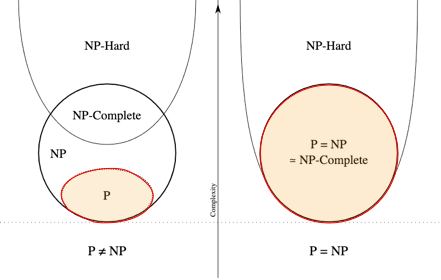
\includegraphics[width=0.7\linewidth]{images/worksheet_7_solution_1.png}
        \end{center}

        \begin{itemize}
            \item Is a class of problems where solution can be guessed and verified
            in polynominal time; non-deterministic means that no particular rule is followed to
            make a guess. $^{[1]}$
            \item Can be verified in ``polynominal'' time
        \end{itemize}

    \end{itemize}

    \bigskip

    \underline{\textbf{References}}

    \bigskip

    \begin{enumerate}[1)]
        \item Encyclopedia Britannica, NP-Complete Problem, \href{https://www.britannica.com/science/NP-complete-problem}{link}
    \end{enumerate}
\end{enumerate}


\end{document}